%%% PG Conf US 2016, NYC
%%%
%%% Lightning talk: pgloader
%%%

\documentclass{beamer}

\usepackage{minted}

\usepackage{beamerthemesplit}
\usepackage[utf8]{inputenc}
%% \usetheme{AnnArbor}
\usetheme{Boadilla}
%% \usetheme{Pittsburgh}
%% \usecolortheme{beaver}
%% \beamertemplatetransparentcovered

\title{pgloader}
\subtitle{PGConf US 2016, NYC}
\author{Dimitri Fontaine \linebreak \url{@tapoueh}}
\date{April 18, 2016}
\logo{
\includegraphics[height=0.4cm]{lbc-logo.png}}

\begin{document}

\frame{\titlepage}

\begin{frame}
  \frametitle{Load data into PostgreSQL. Fast.}

  \center{\url{http://pgloader.io/}}

  \begin{center}
    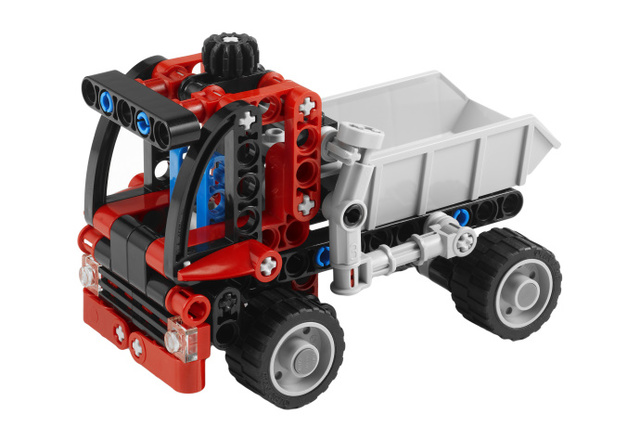
\includegraphics[height=2.1in]{pgloader.jpg}
  \end{center}
\end{frame}

\begin{frame}
  \frametitle{Load data into PostgreSQL. Fast.}

  \center{\url{http://pgloader.io/}}

  \begin{center}
    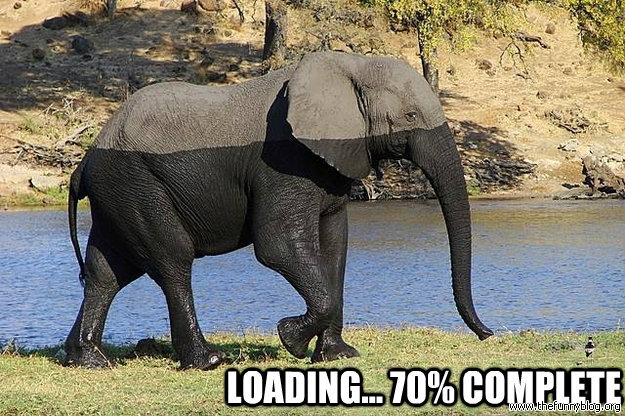
\includegraphics[height=2.1in]{elephant-loading.jpg}
  \end{center}
\end{frame}

\begin{frame}
  \frametitle{pgloader: Open Source, github}

  \center{\url{https://github.com/dimitri/pgloader}}

  \begin{center}
    
\includegraphics[height=2.1in]{Octocat.png}
  \end{center}
\end{frame}

\begin{frame}
  \frametitle{File based formats}

  \begin{columns}[c]
    \column{.5\textwidth}
    \begin{center}
      
\includegraphics[height=6em]{csv_text.png}
    \end{center}
    \column{.5\textwidth}
    \begin{center}
      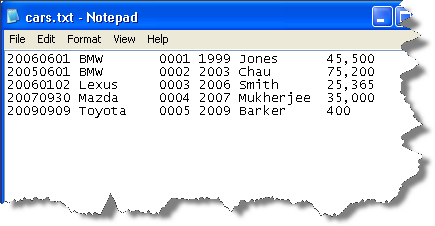
\includegraphics[height=7.5em]{fixedwidthfile.png}
    \end{center}
  \end{columns}
  \vfill

  \begin{columns}[c]
    \column{.5\textwidth} 
    \begin{center}
      
\includegraphics[height=6em]{dBase.png}
    \end{center}
    \column{.5\textwidth}
    \begin{center}
      
\includegraphics[height=6em]{SQLite.png}
    \end{center}
  \end{columns}
\end{frame}

\begin{frame}
  \frametitle{Load from a live connection}

  \center{\url{http://pgloader.io/howto/mysql.html}}
  \vfill
  
  \begin{columns}[c]
    \column{.5\textwidth}
    \begin{center}
      
\includegraphics[height=6em]{mysql.png}
    \end{center}
    \column{.5\textwidth}
    \begin{center}
      
\includegraphics[height=6em]{mssql.png}
    \end{center}
  \end{columns}
\end{frame}

\begin{frame}
  \frametitle{pgloader : Transfom data on the fly}

  \center{\url{http://pgloader.io/}}

  \begin{center}
    
\includegraphics[height=2.1in]{huge-full-outer-join.jpg}
  \end{center}
\end{frame}


\begin{frame}[fragile]
  \frametitle{Using a command language}

  \begin{verbatim}
LOAD CSV
     FROM inline (x, y, a, b, c, d)
     INTO postgresql:///pgloader?csv (a, b, d, c)

     WITH truncate,
          skip header = 1,
          fields optionally enclosed by '"',
          fields escaped by double-quote,
          fields terminated by ','

      SET work_mem to '12MB',
          standard_conforming_strings to 'on'
  \end{verbatim}
\end{frame}

\begin{frame}[fragile]
  \frametitle{with extra before/after sections}

  \begin{verbatim}
   BEFORE LOAD DO
    $$ drop table if exists csv; $$,
    $$ create table csv (
        a bigint,
        b bigint,
        c char(2),
        d text
       );
    $$;
  \end{verbatim}
\end{frame}

\begin{frame}[fragile]
  \frametitle{Some data source examples}

  \begin{verbatim}
  FROM stdin
  FROM inline (a, b, c)
  FROM data/2013_Gaz_113CDs_national.txt
  
  FROM FILENAME MATCHING ~/GeoLiteCity-Location.csv/
  FROM ALL FILENAMES MATCHING ~/ALIOR/
  FROM ALL FILENAMES MATCHING ~/F[A-Z]{4}1[45]|OZ20/
  
  FROM http://www.census.gov/geo/maps-data/
              data/docs/gazetteer/places2k.zip
  
  FROM http://www.insee.fr/fr/methodes/nomenclatures/
                 cog/telechargement/2013/dbf/historiq2013.zip
\end{verbatim}
\end{frame}

\begin{frame}[fragile]
  \frametitle{On the fly data transformations}

  \begin{verbatim}
FROM FILENAME MATCHING ~/GeoLiteCity-Blocks.csv/
     WITH ENCODING iso-8859-1
     (
        startIpNum, endIpNum, locId
     )
INTO postgresql:///ip4r?geolite.blocks
     (
        iprange ip4r using (ip-range startIpNum endIpNum),
        locId
     )
  \end{verbatim}
\end{frame}

\begin{frame}
  \frametitle{On the fly processing useful for CASTing too}

  Empty string and \texttt{NULL}, default values, \textit{zero
    dates} \texttt{0000-00-00}, \texttt{int(11)}, \texttt{float(20,2)},
  \texttt{tinyint} rather than \texttt{boolean}, \texttt{sets}, ...

  \vfill
  \center{Oh, and \textit{\Large encodings} too} \vfill
  
  \begin{center}
    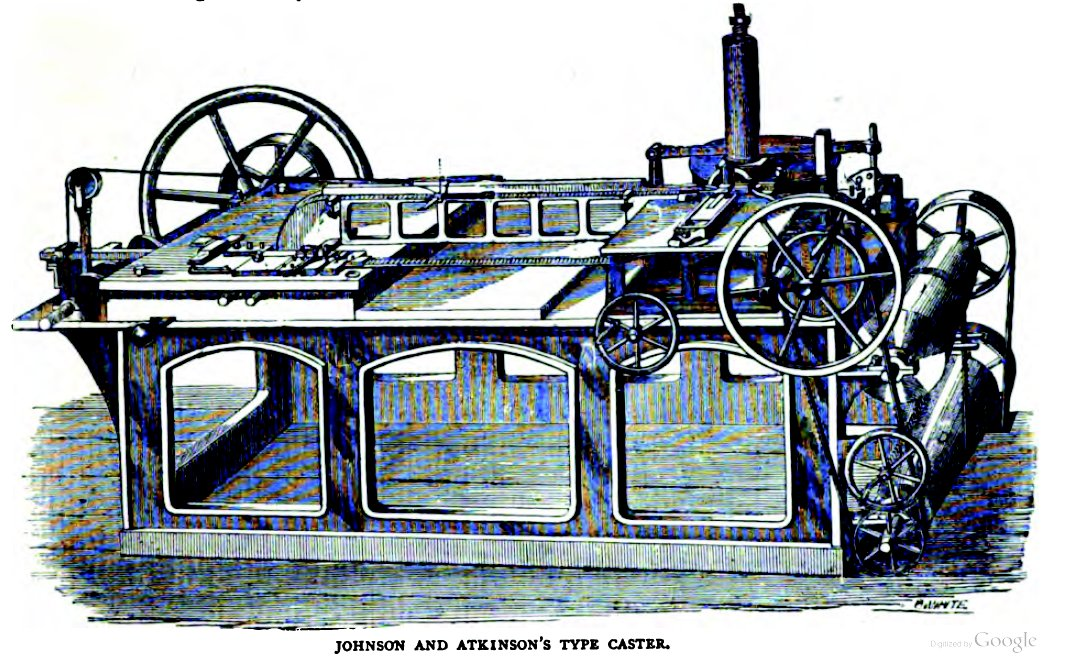
\includegraphics[height=2.1in]{type-casting-machine.jpg}
  \end{center}
\end{frame}

\begin{frame}[fragile]
  \frametitle{Here's how to migrate from MySQL to PostgreSQL}

  \center{\Huge{In \textbf{one} command line.}}
  \vfill

\begin{Verbatim}[fontsize=\Large]
 $ pgloader mysql://user@localhost/sakila \
            pgsql:///pagila
\end{Verbatim}
\end{frame}

\begin{frame}[fragile]
  \frametitle{\small{\texttt{pgloader mysql://root@localhost/sakila pgsql:///pagila}}}

\begin{Verbatim}[fontsize=\tiny]
                   table name       read   imported     errors      total time       read      write
-----------------------------  ---------  ---------  ---------  --------------  ---------  ---------
                  before load          3          3          0          0.008s                     
              fetch meta data         86         86          0          0.184s                     
                 create, drop          0         18          0          0.244s                     
-----------------------------  ---------  ---------  ---------  --------------  ---------  ---------
                        actor        200        200          0          0.011s     0.021s    0.010s
                      address        603        603          0          0.038s     0.040s    0.037s
                     category         16         16          0          0.007s     0.006s    0.007s
                         city        600        600          0          0.037s     0.034s    0.036s
                      country        109        109          0          0.009s     0.026s    0.009s
                     customer        599        599          0          0.022s     0.077s    0.021s
                        films       1000       1000          0          0.052s     0.097s    0.051s
                       ......
                    inventory       4581       4581          0          0.057s     0.190s    0.057s
                     language          6          6          0          0.003s     0.011s    0.003s
                      payment      16049      16049          0          0.246s     0.500s    0.245s
                       rental      16044      16044          0          0.329s     0.623s    0.329s
                        staff          2          2          0          0.025s     0.007s    0.025s
                        store          2          2          0          0.094s     0.010s    0.094s
                   actor_info        200        200          0          0.013s     1.020s    0.012s
             mv.customer_list        599        599          0          0.022s     0.047s    0.022s
                 mv.film_list        997        997          0          0.046s     0.172s    0.046s
-----------------------------  ---------  ---------  ---------  --------------  ---------  ---------
      COPY Threads Completion         69         69          0          2.076s                     
               Create Indexes         41         41          0          0.489s                     
       Index Build Completion         41         41          0          0.002s                     
              Reset Sequences          0         13          0          0.030s                     
                 Primary Keys         16         16          0          0.018s                     
                 Foreign Keys         22         44          0          0.156s                     
             Install comments          0          0          0          0.000s                     
-----------------------------  ---------  ---------  ---------  --------------  ---------  ---------
            Total import time      50086      50086          0          2.788s     3.572s    1.151s
\end{Verbatim}
\end{frame}

\begin{frame}
  \frametitle{And more to come}

  \center{File formats with on-the-fly normalisation}
  
  \begin{columns}[c]
    \column{.5\textwidth}
    \begin{center}
      
\includegraphics[height=9em]{xml.png}
    \end{center}
    \column{.5\textwidth}
    \begin{center}
      
\includegraphics[height=9em]{logo-json.png}
    \end{center}
  \end{columns}
\end{frame}

\begin{frame}
  \frametitle{Other database systems}

  \begin{columns}[c]
    \column{.5\textwidth}
    \begin{center}
      
\includegraphics[height=4em]{oracle-logo.png}
    \end{center}
    \column{.5\textwidth}
    \begin{center}
      
\includegraphics[height=2em]{Informix_d1323_450x450.png}
    \end{center}
  \end{columns}
  \vfill

  \begin{columns}[c]
    \column{.5\textwidth} 
    \begin{center}
      
\includegraphics[height=4em]{mssql.png}
    \end{center}
    \column{.5\textwidth}
    \begin{center}
      
\includegraphics[height=3em]{sybase_logo.png}
    \end{center}
  \end{columns}
\end{frame}

\begin{frame}
  \frametitle{You can become a sponsor!}

  \center{\url{http://pgloader.io/pgloader-moral-license.html}}

  \begin{center}
    
\includegraphics[height=2.1in]{sponsoring.jpg}
  \end{center}
\end{frame}

\begin{frame}
  \frametitle{Load data into PostgreSQL. Fast.}

  \center{\url{http://pgloader.io/}}

  \begin{center}
    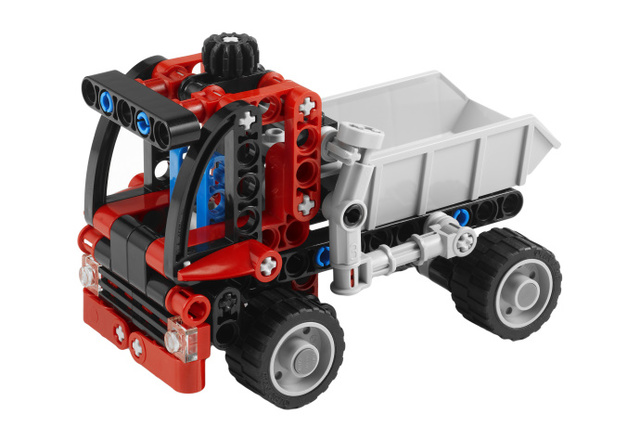
\includegraphics[height=2.1in]{pgloader.jpg}
  \end{center}
\end{frame}

\end{document}
